\subsection{RAID}
Redundant array of independent disks (RAID) is designed as a visualization tool that construct a single storage space with multiple disks. In a RAID system, a file is stripped and stored in different physical disks. A number of variations are evolved to provide different level of data redundancy and I/O performance enhancement \cite{arpaci2012operating}. These variations are \textit{levels}, known as 'RAID' followed by a level number. For example, the most common types of RAID are RAID 0, RAID 1 to RAID 6. Different levels of RAID are differ in their strategies in file striping, mirroring and parity computation. We focus on RAID 6 in this paper.

As a significant advantage compared to the lower levels, RAID 6 is resilient to two arbitrarily disk failure. To be more specific, it is capable of carrying on read and write request to any logic disk despite any two of them are not accessible. Figure \ref{fig:raid6} shows an example of a RAID 6 storage system with data blocks $A, B, C, D$ and $E$, each block is stripped into three parts (1-3) and two parities $p$ and $q$. In the example, parities are being stored in all available disks. An alternative scheme is to store $p$ segments and $q$ segments in two disks separated from the data parts.

\begin{figure}[t]
	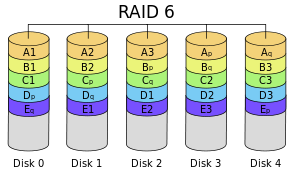
\includegraphics[width=9cm,height=5cm,angle=0]{RAID6.png}
	\caption{Diagram of a RAID 6 storage system with 3 block level data strippings and 2 parities \cite{wiki:raid} }
	\label{fig:raid6}
\end{figure}


\subsection{Erasure Coding}

Erasure coding is the technique used to encode data into data plus codings, so the original contents are recoverable when disks with data fail. More formally, for a given $k$ disks space of data, erasure coding creates $k+m$ disks of data, where $m$ disks are codings or parities. So when up to $m$ disks fail, the contents are recoverable by decoding the erasure code. In the example from Figure \ref{fig:raid6}, a specific erasure coding algorithm can be used to calculate from three disks of data to produce $3+2=5$ disks of data and stored in five disks, where parities $p$ and $q$ are codings information that is essential for data recovery. So when up to 2 disks fail, data access is not affected.


%\subsection{Galois field}
%The first parity in RAID 6 is usually computed with a $XOR$ operation, while the other is preferred to be computed in a Galois field. Galois Field is a finite field that the size of membership is limited to $p^k$, where $p$ is a prime number and $k$ is a positive integer. 
%
%For example, the range of valid numbers in a Galois field $GF(2^8)$ is $0$ to $2^8-1=255$, and the 


\subsection{Reed-Solomen Coding}

In general, there are two main strategies to guarantee certain level of fault-tolerance. The first is full duplication, where all storage nodes have a independent mirror backup. In case of access failure, the backup copy can be used. The advantage of such design is, for a single fault, data recovery takes exactly the same read as the original request, incurring no additional read overhead. However, it is less cost-efficient, using only $1/2$ of the total hardware effectively in data storage. The second is using erasure coding.

One popular erasure coding scheme is Reed–Solomon coding. It is a error correction coding that has been widely used in communication and storage systems.